\chapter{Introduction}
Abstract algebra is the study of algebraic structure that came into existence in
early nineteenth century as complex problems and solutions evolved in other
branch of mathematics such as geometry, number theory and polynomial equations.
Being relatively new subject in mathematics, algebraic structures are used in
various fields. For example, \cite{liaqat2021some} use semigroup \footnotetext{A
kind of algebraic structure} to study time dependent partial differential
equations in technique similar to differential equations on a function space.
Kleene algebra, semigroup structures are used in finite automata to better model
and understand the finite state machines. \textit{Groups} are one of the oldest
structures that are used in number theory, in atomic and molecular theory,
cryptography \cite{enwiki:1133598242}. \cite{bruck1944some} uses
\textit{Quasigroups} and \textit{loops} structures for encryption of image data.
The simplest algebraic structure is magma. A magma has a set with a binary
operation that is closed by definition. A magma with associative property is
called a semigroup. Magma with division operation is called a quasigroup. Figure
\ref{fig_magma} shows the algebra hierarchy from magma to group. 
 \begin{figure}[ht]
	\centering
	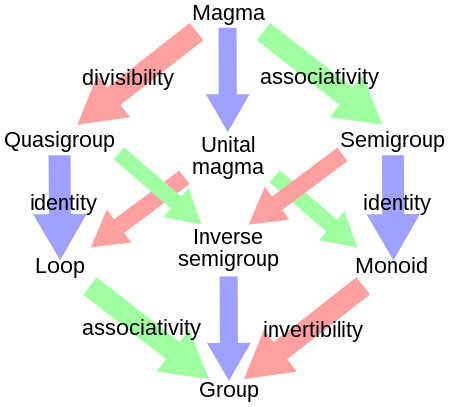
\includegraphics[width=0.7\textwidth]{figures/Sample/Magma_to_group.jpg}
	\caption{Algebraic structure hierarchy \cite{enwiki:1107380309}}
	\label{fig_magma}
 \end{figure}

With growing help of technology, mathematicians are more indulged in automated
reasoning. Increasing powers of computers, software tools that help towards
automated reasoning becomes useful in their research. Although the proof systems
that support first-order logic are successful, developing a tool that supports
higher order logic is complex \cite{phillips2010automated} and requires
carefully defining mathematical objects and concept. Proof assistant systems act
as a bridge between computer intelligence and human effort in developing
mathematical proofs. Agda, Coq, Isabelle, Lean and Idris are some commonly used
proof assistant systems. Mathematicians use these proof assistants to check their
proof for validity, build proofs and sometimes even generate them via proof
search tools  For the scope of the thesis we only discuss algebraic
structures in proof systems.

\section{Research Outline}
For any software system to be robust, all its dependencies must similarly be
robust. The standard libraries of these systems should support the user with all
necessary functionalities to be able to use the system easily without having to
define all functionalities. To generate robust libraries of knowledge, the
author of \cite{BuildingDiamond} explore technique to generate libraries with
minimum human efforts. However, while their methods do work in theory, they are
difficult (and expensive) in practice. Although, generated libraries can define
the algebraic concepts required, they are not fully reliable and hence not
considered as "standard library" for any proof system. For now, building
standard libraries for proof systems rely on human efforts. This led to the
question of what is the current scope of algebraic structures in the proof
assistant systems. A survey was conducted to better understand the coverage of
algebra in four proof systems Agda, Idris, Lean and Coq. Agda was one such
system where there was better scope to contribute to the standard library.
\footnote{I was exposed to Agda during course work for my Master's degree,
further adding bias to choosing Agda over other systems} 

As part of this thesis, more than twenty-three structures was defined in the
standard library for Agda. Inspired by the ways algebraic structures are used in
research, in this work we explore capturing a select subset of them in Agda
standard library. Following the algebra hierarchy in Figure ~\ref{fig_magma}, we
study magma with division operations that is quasigroup and loop structures. We
also explore various types of loop such as bol-loop and moufang-loop and their
properties. Quasigroup only have weak associative property and do not have
inverse. In order to have well-defined inverse, the structure should have
associative property. Semigroup is the simplest structure with associative
property and are used in various fields such as probability theory and formal
systems. One of the most commonly studied algebraic structure is Ring. In this
thesis we study types of rings such as near-ring, quasi-ring and non-associative
ring. Along with ring structure, the most used structure is Kleene algebra. The
applications of Kleene algebra is seen in finite state machines, regular
expressions and other branch of computer science. As part of this thesis, we
study Kleene algebra by providing proofs for its properties that may be used in
developing other systems or in applications. By contributing to Agda standard
library, we hope that this work will be used by others. 

Notably, as we explore capturing these structures in Agda, we analyze five problems that arise:
\begin{enumerate}
\item Ambiguity in naming structures.
\item Equivalent structures that are structurally different.
\item Redundant field during structural inheritance.
\item Identical structures that can be derived in many ways in algebra hierarchy
\item Equivalent structures that are structurally same.
\end{enumerate}
To overcome these problems we explore the use of \textit{product family
algebra}.

\section{Thesis Outline}
Chapters 2 and 3 focus on background information necessary for reading this
work, focusing on reviewing universal algebra and algebraic structures in Agda,
respectively. Chapter 4 justifies the scope of the thesis contribution by a
survey on algebraic coverage in proof systems. The next three chapters 5,6 and 7
are dedicated to discuss the structures in details. Chapter 5 explores
quasigroup and loop structures that uses division operation. Chapter 6 discusses
the properties of semigroup and rings with variations of ring structure. Chapter
7 explores Kleene algebra, definition, construct and properties in Agda. Chapter
8 describes the various problems we faced during this work, as well as advice on
handling common issues in programming algebras in proof systems. Finally,
Chapter 9 concludes this work with notes on related future works and some
closing thoughts.
